

\lstdefinelanguage{bash}{
	keywords={ls, cd, echo, cat, mkdir, rm, cp, mv, chmod, chown, grep, find},
	sensitive=true,
	morecomment=[l]{\#},
	morestring=[b]",
}

\lstset{
	language=bash,
	basicstyle=\ttfamily\small,
	keywordstyle=\color{blue},
	stringstyle=\color{green!50!black},
	commentstyle=\color{gray},
	showstringspaces=false,
	frame=single,
	breaklines=true
}


\chapter{Implementation}

This chapter presents the technical realisation of the AI-GCode-Generation project, describing how the pipeline was implemented in practice. The section proceeds from environment setup and installation of libraries, through orchestration of agents, to the execution of the complete workflow. Selected code examples are included where they are essential for understanding.

\section{Project Setup and Installation}
The project was implemented in Python 3.12, making use of specialized libraries for computer vision, SVG handling, and G-code generation. To ensure reproducibility, a \texttt{requirements.txt} file was prepared containing all necessary dependencies.

\subsection{Clone Repository}
The codebase is organized as a modular agent-based system, accessible through the project repository. To begin, the repository is cloned locally~\ref{lst:Clone}:

\begin{lstlisting}[language=bash,caption={Clone Repository}, label={lst:Clone}]
	#!/bin/bash
	# Clone the Repository
	git clone https://github.com/mahajan-vatsal/AI-GCode-Generation.git
	cd AI-GCode-Generation
\end{lstlisting}

\subsection{Python Environment}
A dedicated virtual environment ensures isolation and compatibility ~\ref{lst:Python} :

\begin{lstlisting}[language=bash,caption={Create Virtual Environment}, label={lst:Python}]
	#!/bin/bash
	# Create the Virtual environment
	python3.12 -m venv venv
	source venv/bin/activate   # macOS/Linux
	venv\Scripts\activate      # Windows
\end{lstlisting}

\subsection{Install Dependencies}
The required libraries are installed from the provided \texttt{requirements.txt} file ~\ref{lst:text} :

\begin{lstlisting}[language=bash,caption={Install Dependencies}, label={lst:text}]
	#!/bin/bash
	# Install required dependencies
	pip install -r requirements.txt
\end{lstlisting}

This installs core packages including LangGraph, OpenCV, svgwrite, cairosvg, svg2gcode, and AI model connectors such as OpenRouter and Fireworks APIs.

\subsection{Listing APIs}
API keys are managed via a .env file to ensure secure access to external models ~\ref{lst:evn} :

\begin{lstlisting}[language=bash,caption={APIs Listing}, label={lst:evn}]
	#!/bin/bash
	# Listing all the necessaries APIs
	# Fireworks (OpenAI) for OCR and layout detection
	FIREWORKS_API_KEY=your_fireworks_key_here
	# OpenRouter (Mistral) for generating SVG edit commands
	OPENROUTER_API_KEY=your_openrouter_key_here
	#Langgraph for defining the Workflow
	LANGCHAIN_PROJECT=AI-GCode-Generator
	export LANGCHAIN_API_KEY=your_langchain_key_here
	export LANGCHAIN_ENDPOINT=https://api.smith.langchain.com
	LANGSMITH_TRACING=true
	LANGSMITH_PROJECT=AI-GCode-Generator
\end{lstlisting}

\section{Running the LangGraph Workflow}
The orchestration of the pipeline is managed by \texttt{LangGraph}, which interprets the defined workflow in \texttt{main\_graph.py} and \texttt{subgraph.py}

\subsection{Start LangGraph Server}
LangGraph provides a local development server for executing workflows ~\ref{lst:server} :
\begin{lstlisting}[language=bash,caption={Langgraph Server}, label={lst:server}]
	#!/bin/bash
	# Start the Langraph Server
	langgraph dev
\end{lstlisting}

This command launches the workflow as defined in \texttt{langgraph.json}, where the entry point \texttt{main\_graph.py:graph\_app} specifies the top-level pipeline.

\subsection{Workflow Execution}
Once the server is active, the workflow can be initiated with an input business card image (e.g., \texttt{.jpg} or \texttt{.png}) ~\ref{lst:input} as show in fig. ~\ref{Input}. . The pipeline then proceeds through the following stages. 

\begin{enumerate}
	\item OCR and Layout Detection
	\item SVG Generation
	\item SVG Editing and Preview
	\item Rasterisation and Binarisation
	\item G-code Generation and Preview
\end{enumerate}

\begin{lstlisting}[language=bash,caption={Sample Input},label={lst:input}]
	{"image_path": "samples/business_card3.png"}
\end{lstlisting}

\begin{figure}
	\begin{center}
		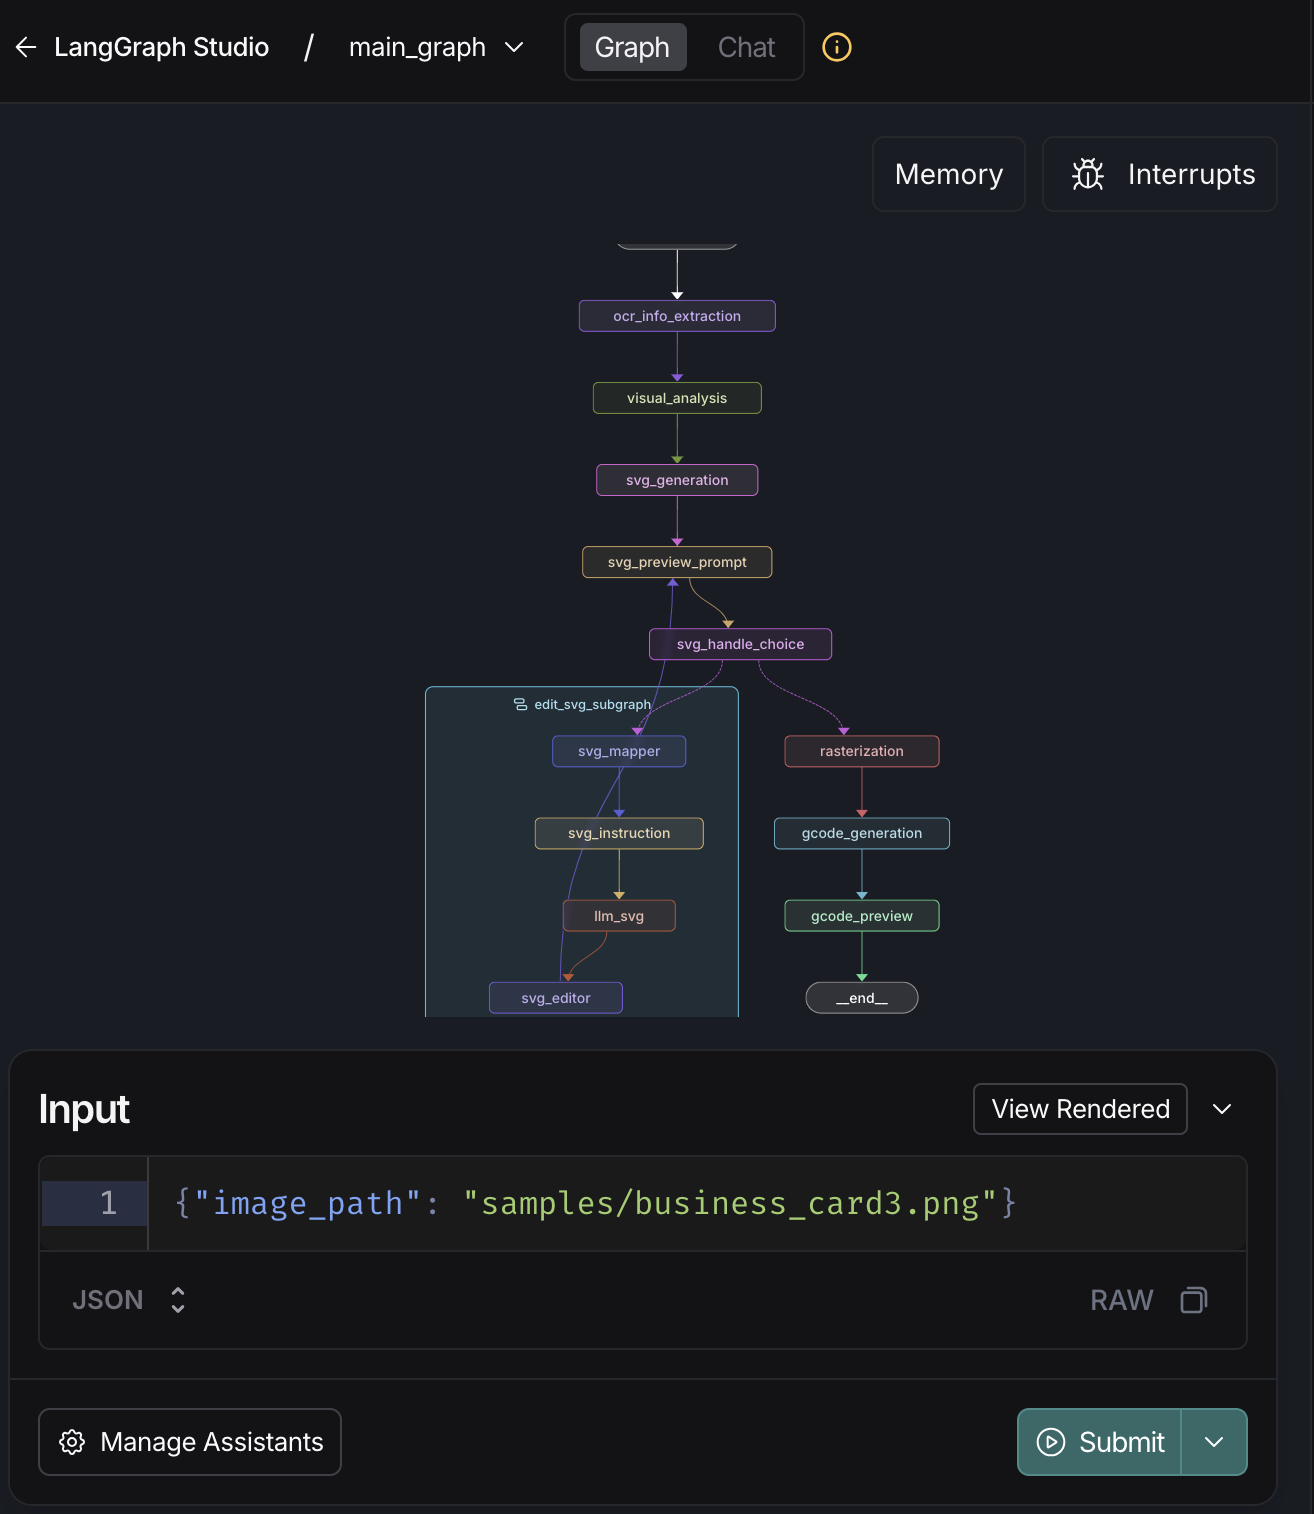
\includegraphics[width=0.6\linewidth]{Images/Input.png}
		\caption{Sample Input}
		\label{Input} 
	\end{center}
\end{figure}

\section{Agent-Level Implementation}

\subsection{OCR Agent}

 \begin{itemize}	
\item \textbf{Purpose}: Extracts structured textual data (names, phone numbers, emails, addresses) from the card image using Fireworks API (Qwen2.5-VL).
\item \textbf{Implementation:} Defined in \texttt{ocr\_agent.py}, it preprocesses the image via OpenCV and invokes the vision-language model for recognition.
\item \textbf{Output:} JSON structure with extracted text fields as shown in fig.~\ref{OCR} .
\end{itemize}

\begin{figure}
	\begin{center}
		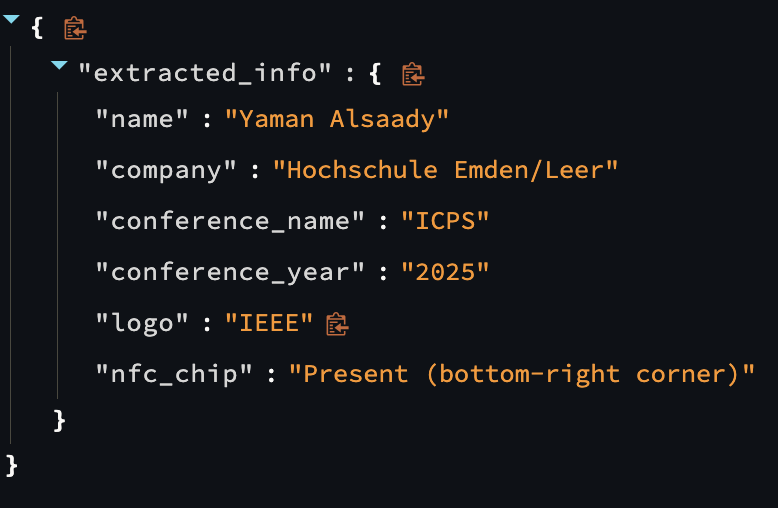
\includegraphics[width=0.5\linewidth]{Images/ocr.png}
		\caption{Node OCR JSON Output}
		\label{OCR} 
	\end{center}
\end{figure}


\subsection{Visual Analysis Agent}
\begin{itemize}
	\item \textbf{Purpose:} Detects logos, QR codes, NFC chips, and text block bounding boxes.
	\item \textbf{Implementation:} Uses OpenCV contour analysis and Qwen2.5-VL for semantic enrichment in \texttt{visual\_analysis\_agent.py}.
	\item \textbf{Output:} Bounding box coordinates converted to millimetre space (85 $\times$ 54 mm) ~\ref{Visual}.
\end{itemize}

\begin{figure}
	\begin{center}
		\includegraphics[width=0.4\linewidth]{Images/Visual.png}
		\caption{Node Visual JSON Output}
		\label{Visual} 
	\end{center}
\end{figure}

\subsection{SVG Agent}
\begin{itemize}
	\item \textbf{Purpose:} Generates a Scalable Vector Graphics (SVG) file representing the card layout.
	\item \textbf{Implementation:}
	\begin{itemize}
		\item Text placed using \texttt{<text>} elements.
		\item Logos or QR codes embedded with \texttt{<image>} or \texttt{<path>}.
		\item Coordinates flipped to match SVG’s top-left coordinate system.
	\end{itemize}
	\item \textbf{Library Used:} \texttt{svgwrite} for programmatic construction.
	\item \textbf{Output:} \texttt{output.svg} ~\ref{SVG}.
	
	\begin{figure}
		\begin{center}
			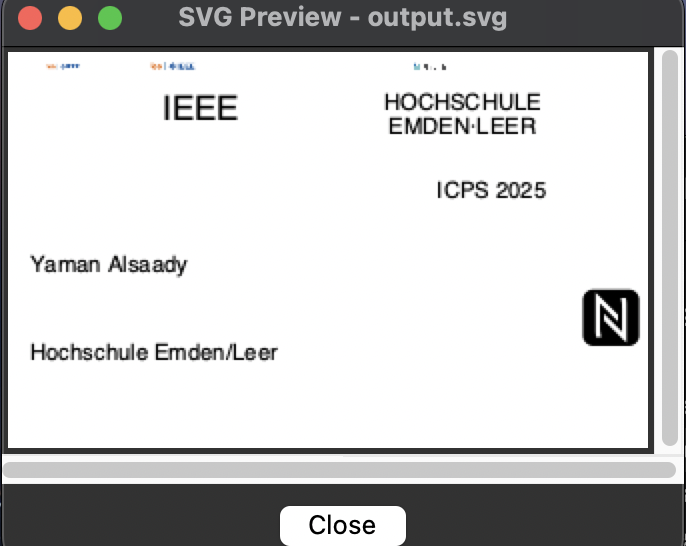
\includegraphics[width=0.6\linewidth]{Images/svg.png}
			\caption{Node SVG Output}
			\label{SVG} 
		\end{center}
	\end{figure}
\end{itemize}

\subsection{Editing \& Preview Agents}
\begin{itemize}
	\item \textbf{LLM-SVG Agent (\texttt{llm\_svg\_agent.py}):}
	\begin{itemize}
		\item Converts natural language edit commands (e.g., “Replace 'Yaman' with 'Vatsal'. or add\_text tagline at x=10 y=6 text='Created by Vatsal' size=3.2”) into structured SVG modifications.
		\item Uses Mistral 7B via OpenRouter.
	\end{itemize}
	\item \textbf{SVG Editor Agent (\texttt{svg\_editor\_agent.py}):}
	\begin{itemize}
		\item Applies parsed commands (move, replace, delete, add\_text).
	\end{itemize}
	\item \textbf{SVG Preview Agent (\texttt{svg\_preview\_agent.py}):}
	\begin{itemize}
		\item Provides GUI preview of the card in Tkinter, enabling human-in-the-loop validation.
	\end{itemize}
		\item \textbf{Output} 
		\begin{itemize}
		\item After applying the editing instructions the SVG file looks like ~\ref{edit}. 
				\begin{figure}
			\begin{center}
				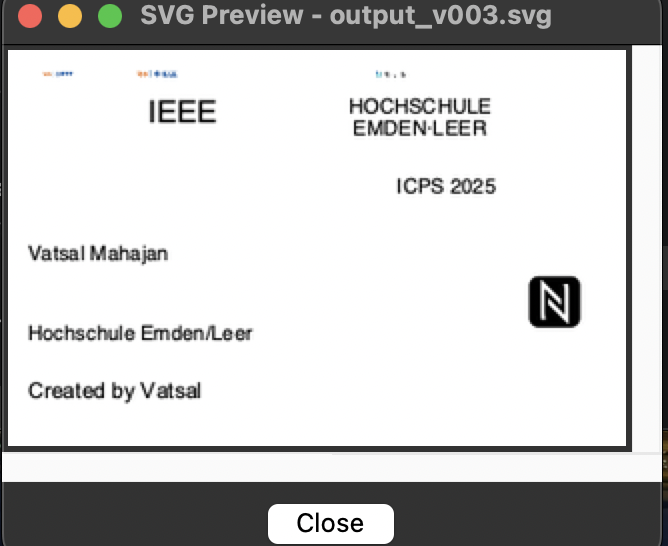
\includegraphics[width=0.6\linewidth]{Images/edit.png}
				\caption{Node SVG-Edited Output}
				\label{edit} 
			\end{center}
		\end{figure}
		\end{itemize}
	
\end{itemize}

\subsection{Rasterisation Module}
\begin{itemize}
	\item \textbf{Purpose:} Converts SVG into a high-resolution PNG, then applies binarisation to produce a black-and-white engraving-ready bitmap.
	\item \textbf{Implementation:} \texttt{rasterization.py} uses CairoSVG + OpenCV for conversion.
	\item \textbf{Output:} \texttt{output\_bw.png} ~\ref{raster}.
	
		\begin{figure}
		\begin{center}
			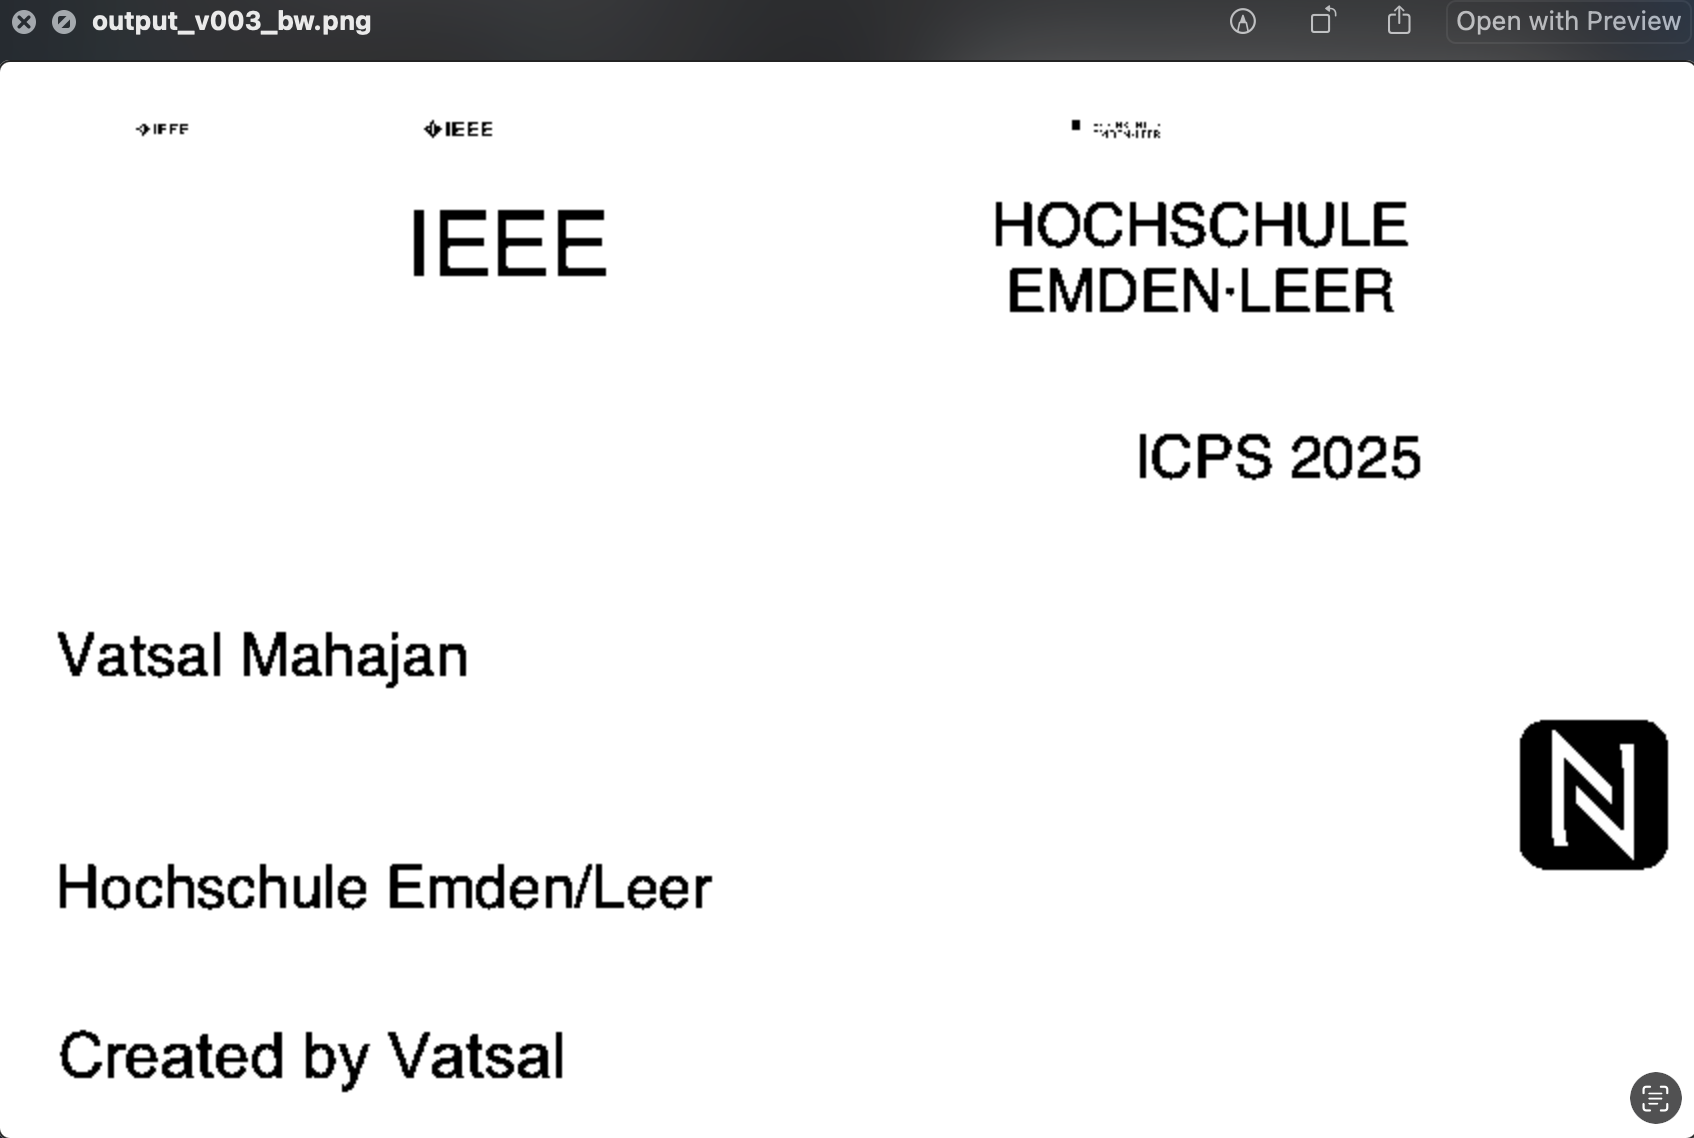
\includegraphics[width=0.5\linewidth]{Images/raster1.png}
			\caption{Node Rasterisation Output}
			\label{raster} 
		\end{center}
	\end{figure}
\end{itemize}



\subsection{G-code Agent \& Preview}
\begin{itemize}
	\item \textbf{Purpose:} Translates the binarised bitmap into scanline G-code.
	\item \textbf{Implementation:}
	\begin{itemize}
		\item \texttt{gcode\_agent.py} generates line-by-line motion instructions (G0, G1, laser ON/OFF).
		\item Raster scanning implemented as zig-zag passes for efficiency.
	\end{itemize}
	\item \textbf{Preview:} \texttt{gcodePreview\_agent.py} displays toolpaths with Tkinter as shown in fig ~\ref{GcodeP}.
	\item \textbf{Output:} \texttt{output.gcode} ~\ref{Gcode}.

		
\end{itemize}

			\begin{figure}
	\begin{center}
		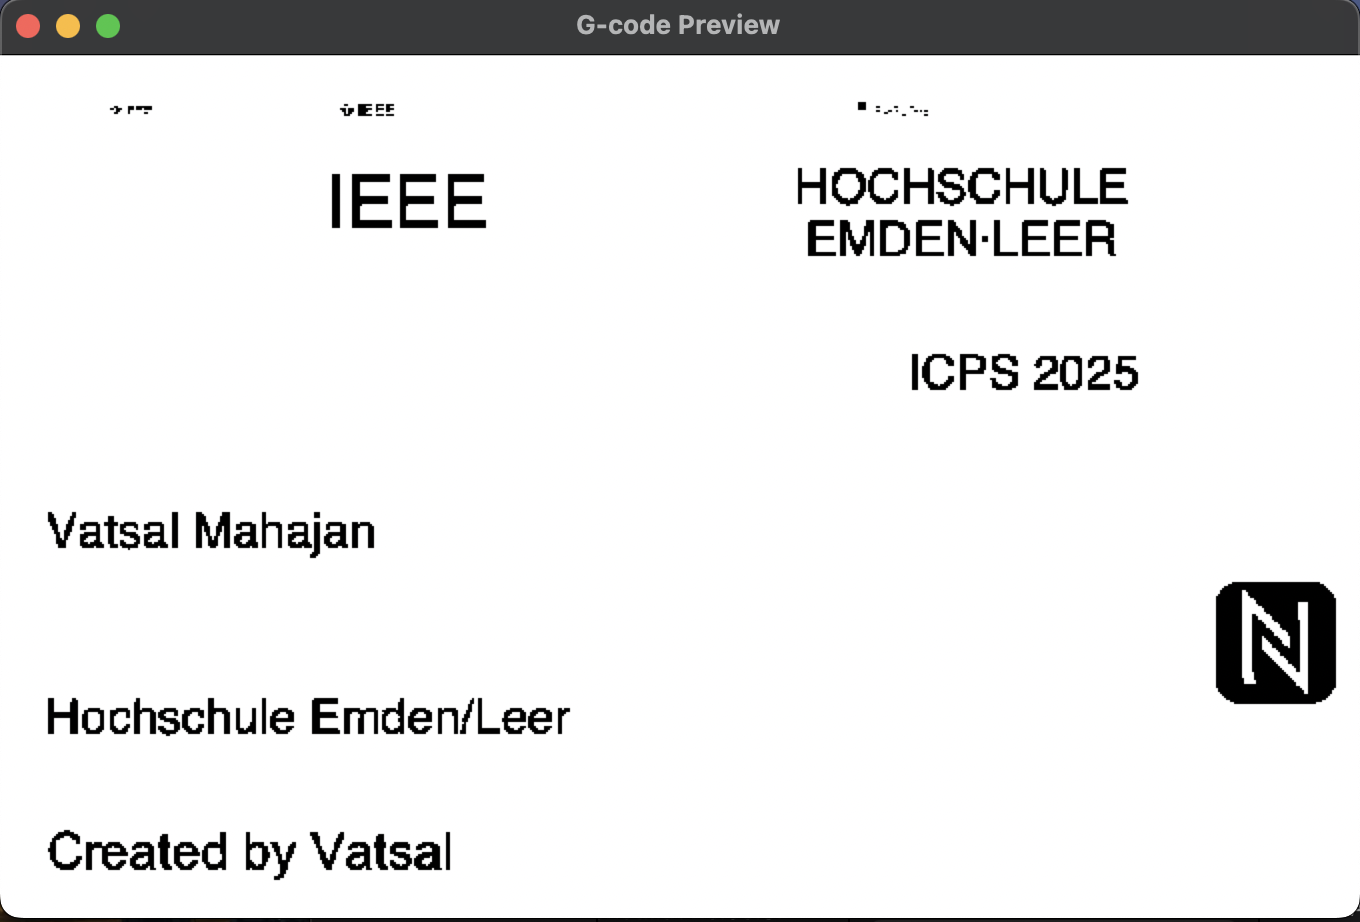
\includegraphics[width=0.6\linewidth]{Images/GcodeP.png}
		\caption{Node Gcode Preview Output}
		\label{GcodeP} 
	\end{center}
\end{figure}

\begin{figure}
	\begin{center}
		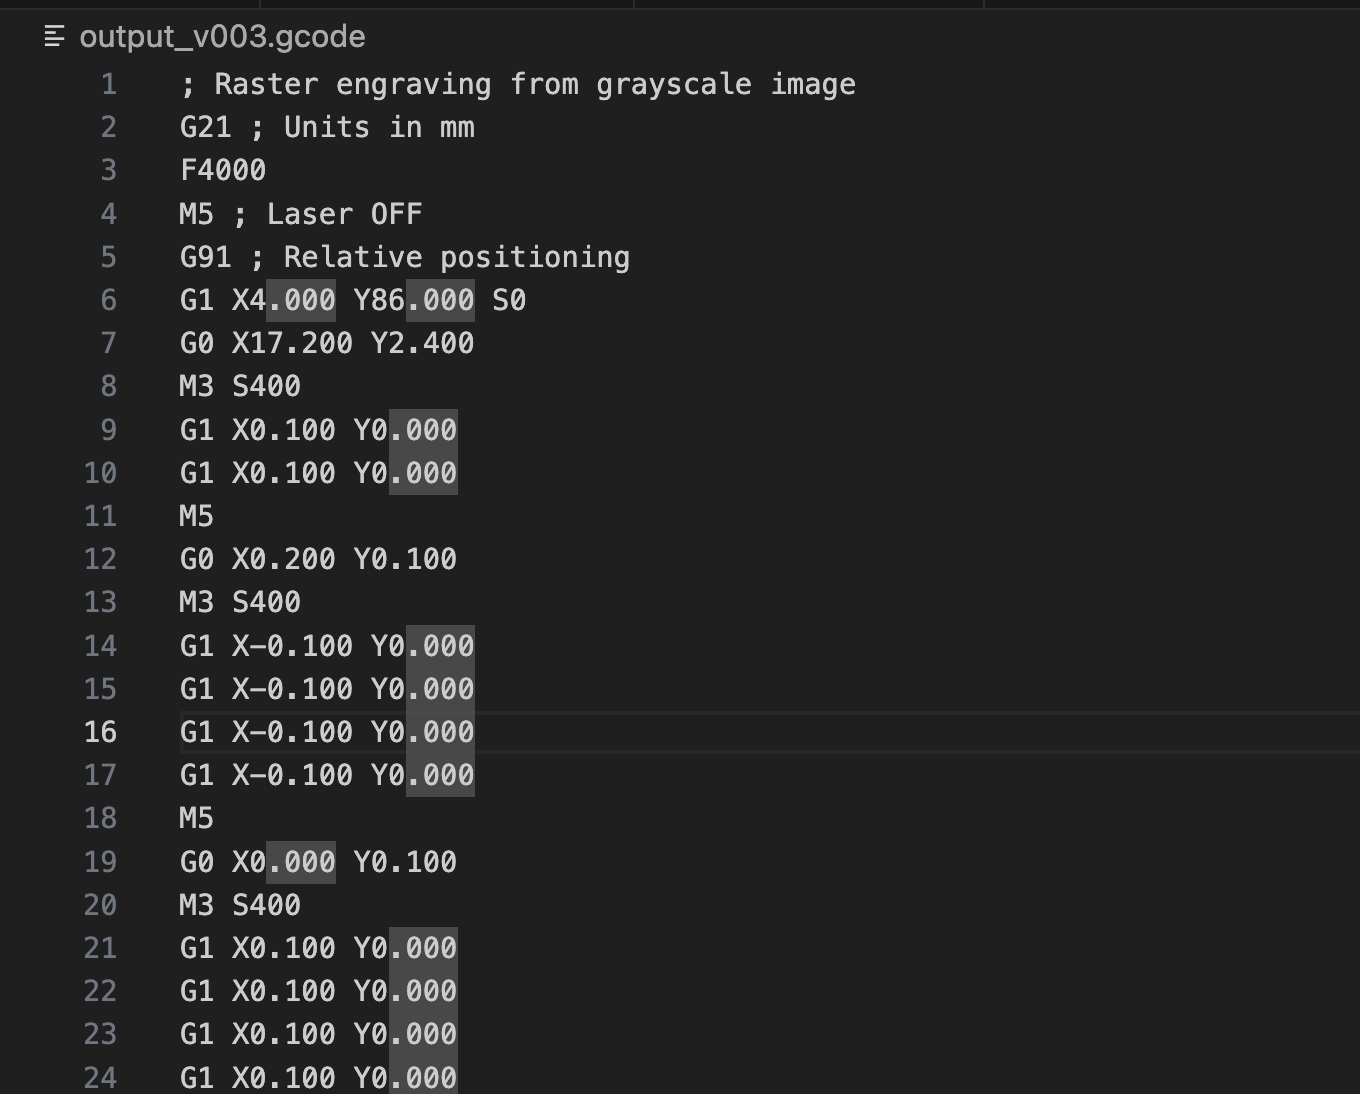
\includegraphics[width=0.6\linewidth]{Images/Gcode.png}
		\caption{Node Gcode Generate Output}
		\label{Gcode} 
	\end{center}
\end{figure}

\subsection{Human-in-the-Loop Integration}
\begin{itemize}
	\item At two stages, the system pauses for optional human input:
	\begin{enumerate}
		\item \textbf{User Input} – Asking from Users whether they wanted to edit the svg or proceed to generate GCode ~\ref{user}.
		\item \textbf{SVG Editing} – User may issue natural language commands to reposition or replace elements ~\ref{svg-edit}.
		\end{enumerate}
		
					\begin{figure}
			\begin{center}
				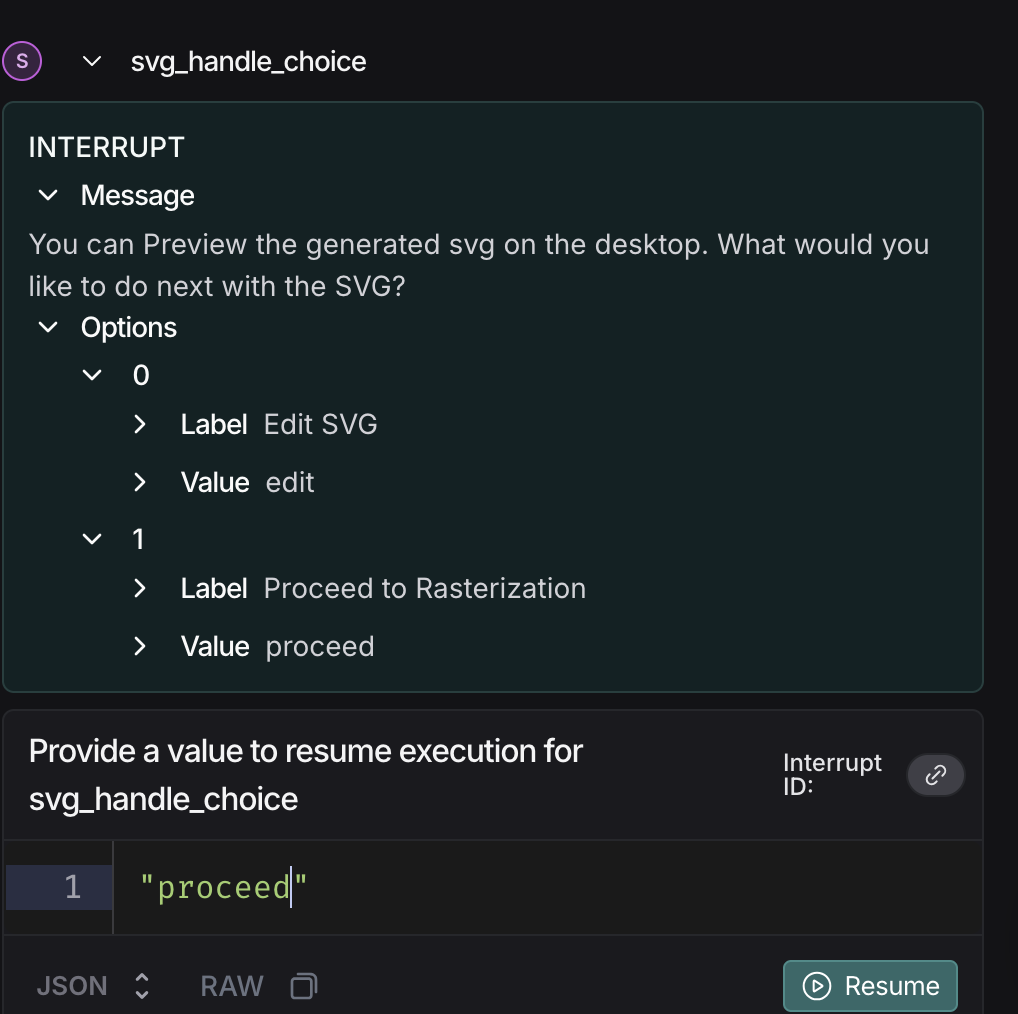
\includegraphics[width=0.6\linewidth]{Images/user-input.png}
				\caption{Asking User choice}
				\label{user} 
			\end{center}
		\end{figure}
		
		\begin{figure}
			\begin{center}
				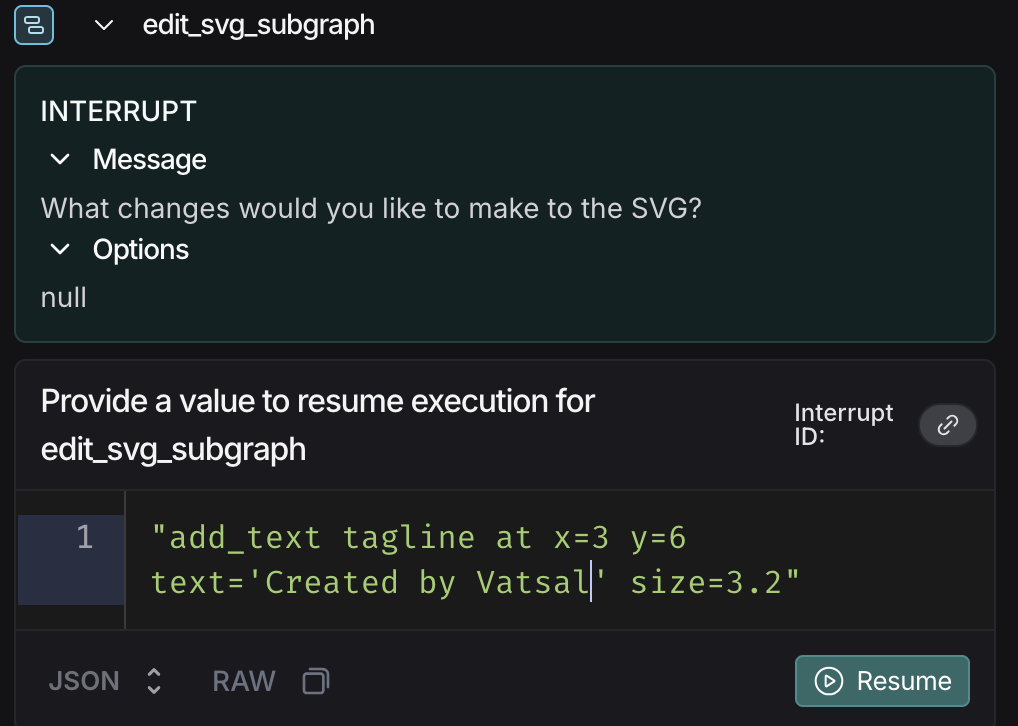
\includegraphics[width=0.6\linewidth]{Images/svg-edit.png}
				\caption{Instruction for editing}
				\label{svg-edit} 
			\end{center}
		\end{figure}
		
	\item This hybrid approach combines automation for efficiency with manual oversight for reliability, aligning with best practices in AI-assisted manufacturing.
\end{itemize}

\section{Web User Interface Implementation}
\subsection{Purpose of the Web UI}
While the backend pipeline orchestrates OCR, layout analysis, SVG generation, rasterisation, and G-code creation, it is equally important to provide users with an accessible interface. To address this, a lightweight web-based user interface (UI) was developed, enabling interaction with the system without requiring direct command-line operations. This UI lowers the technical barrier for end-users and aligns with human-machine interaction principles commonly adopted in digital manufacturing environments.

\subsection{Tools and Frameworks}
The web UI was built using:
\begin{itemize}
	\item \texttt{streamlit.py}: Provides a rapid, Python-based framework for building interactive web applications. It enables file upload, dynamic visualisation, and step-by-step user workflows .
	\item \texttt{server\_api.py}: Implements REST-style endpoints to connect the front end with the backend agents. User actions (e.g., upload or edit requests) are translated into API calls.
	\item \texttt{server\_hmi.py}: Functions as the Human-Machine Interface (HMI) layer, bridging user interactions with backend orchestration.
	\item LangGraph Integration: The UI triggers LangGraph nodes to perform OCR, SVG editing, and G-code generation, ensuring a consistent workflow across both backend automation and frontend interactivity
\end{itemize}

\subsection{Advantages of the Web UI}
\begin{itemize}
	\item \textbf{Accessibility:} Users without programming expertise can run the full engraving pipeline.
	\item \textbf{Transparency:} Intermediate previews (SVG, raster image, G-code) are exposed, enhancing trust and reducing risk of errors.
	\item \textbf{Integration with Digital Factory:} The UI demonstrates how an AI-driven engraving module can be operated as part of a larger smart factory setup, with clear potential for extension to mobile or remote control interfaces
	
\end{itemize}

\subsection{Triggering the Web UI}
To enable accessibility, the Web UI can be triggered directly from the project environment without requiring complex setup. After installing dependencies and configuring API keys in the  \texttt{.env} file (see Section 3.1.3), the following commands launch the user interface:

\subsubsection{Start the Backend API Server}

\begin{lstlisting}[language=bash,caption={Start backend Server}, label={lst:backend}]
uvicorn server\_api:app --host 0.0.0.0 --port 8080
\end{lstlisting}

\begin{itemize}
	\item \textbf{unicorn:} A lightweight ASGI server for running FastAPI or similar Python apps.
	\item \textbf{server\_api:app:} Load the file \texttt{server\_api.py} and Inside that file, find the object named app (usually a FastAPI instance).
	\item \textbf{--host 0.0.0.0:} Binds the server to all available network interfaces (not just localhost). This allows access from other machines on the same network (e.g., from another PC or Raspberry Pi).
	\item \textbf{--port 8080:} The backend server listens for HTTP requests on port 8080.
\end{itemize}
This starts your backend API layer ~\ref{unicorn}, exposing endpoints like /upload, /process\_svg, /generate\_gcode, etc.

\begin{figure}
	\begin{center}
		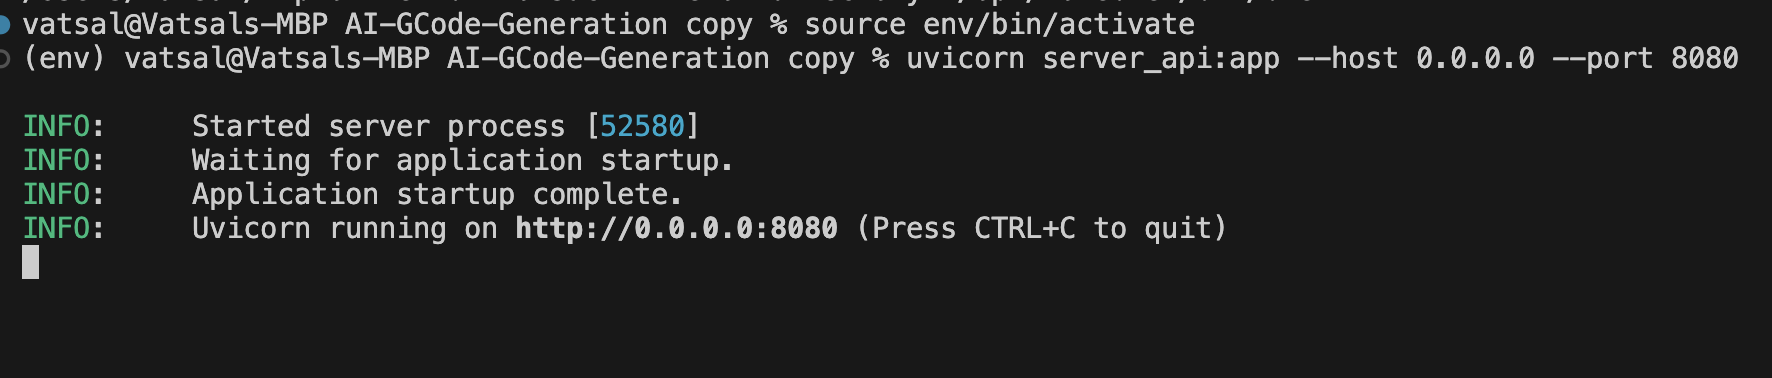
\includegraphics[width=1\linewidth]{Images/unicorn.png}
		\caption{Backend Output}
		\label{unicorn} 
	\end{center}
\end{figure}


\subsubsection{Frontend Web UI}
In another terminal write the following command and in the terminal it looks like ~\ref{streamlit}:
\begin{lstlisting}[language=bash,caption={Start Frontend Web UI}, label={lst:Frontend}]
	streamlit run streamlit.py --server.address 0.0.0.0 --server.port 8501
\end{lstlisting}


\begin{figure}
	\begin{center}
		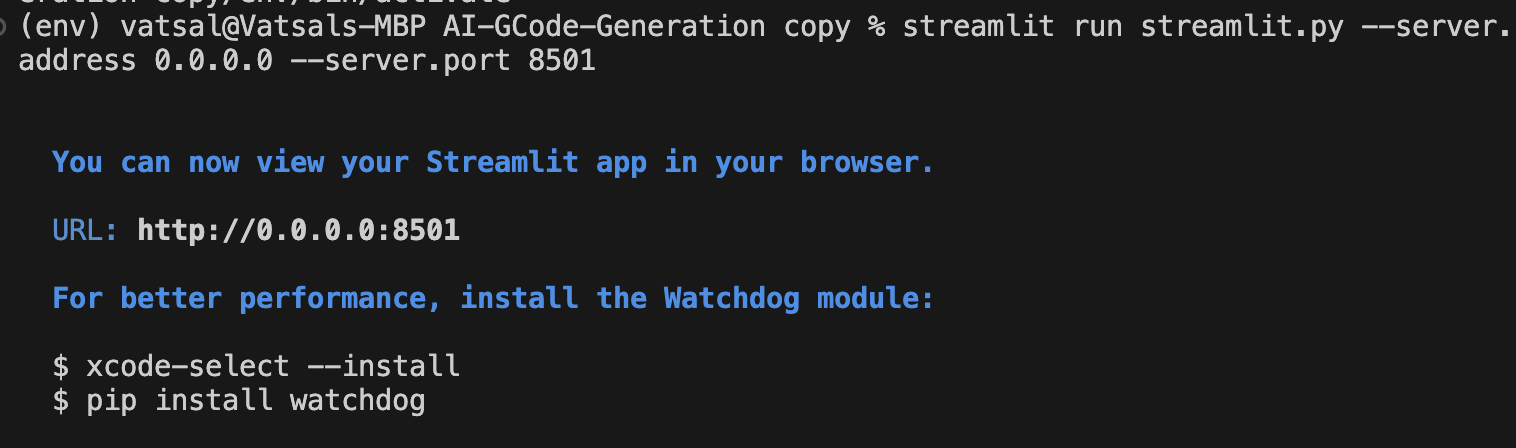
\includegraphics[width=1\linewidth]{Images/streamlit.png}
		\caption{Frontend Output}
		\label{streamlit} 
	\end{center}
\end{figure}

\begin{itemize}
	\item \textbf{streamlit run streamlit.py:} Launches the file \texttt{streamlit.py} as a Streamlit web app.
	\item \textbf{--server.address 0.0.0.0:} Makes the app accessible on all network interfaces (so not just localhost:8501, but also \texttt{http://<your\_machine\_ip>:8501)}, So that other can also access.
	\item \textbf{--server.port 8501:} Runs the app on port \texttt{8501} (default Streamlit port).
\end{itemize}
This starts your user-facing UI as shown in fig. ~\ref{WebUI}, where users can upload cards, preview results, and trigger backend calls.

\begin{figure}
	\begin{center}
		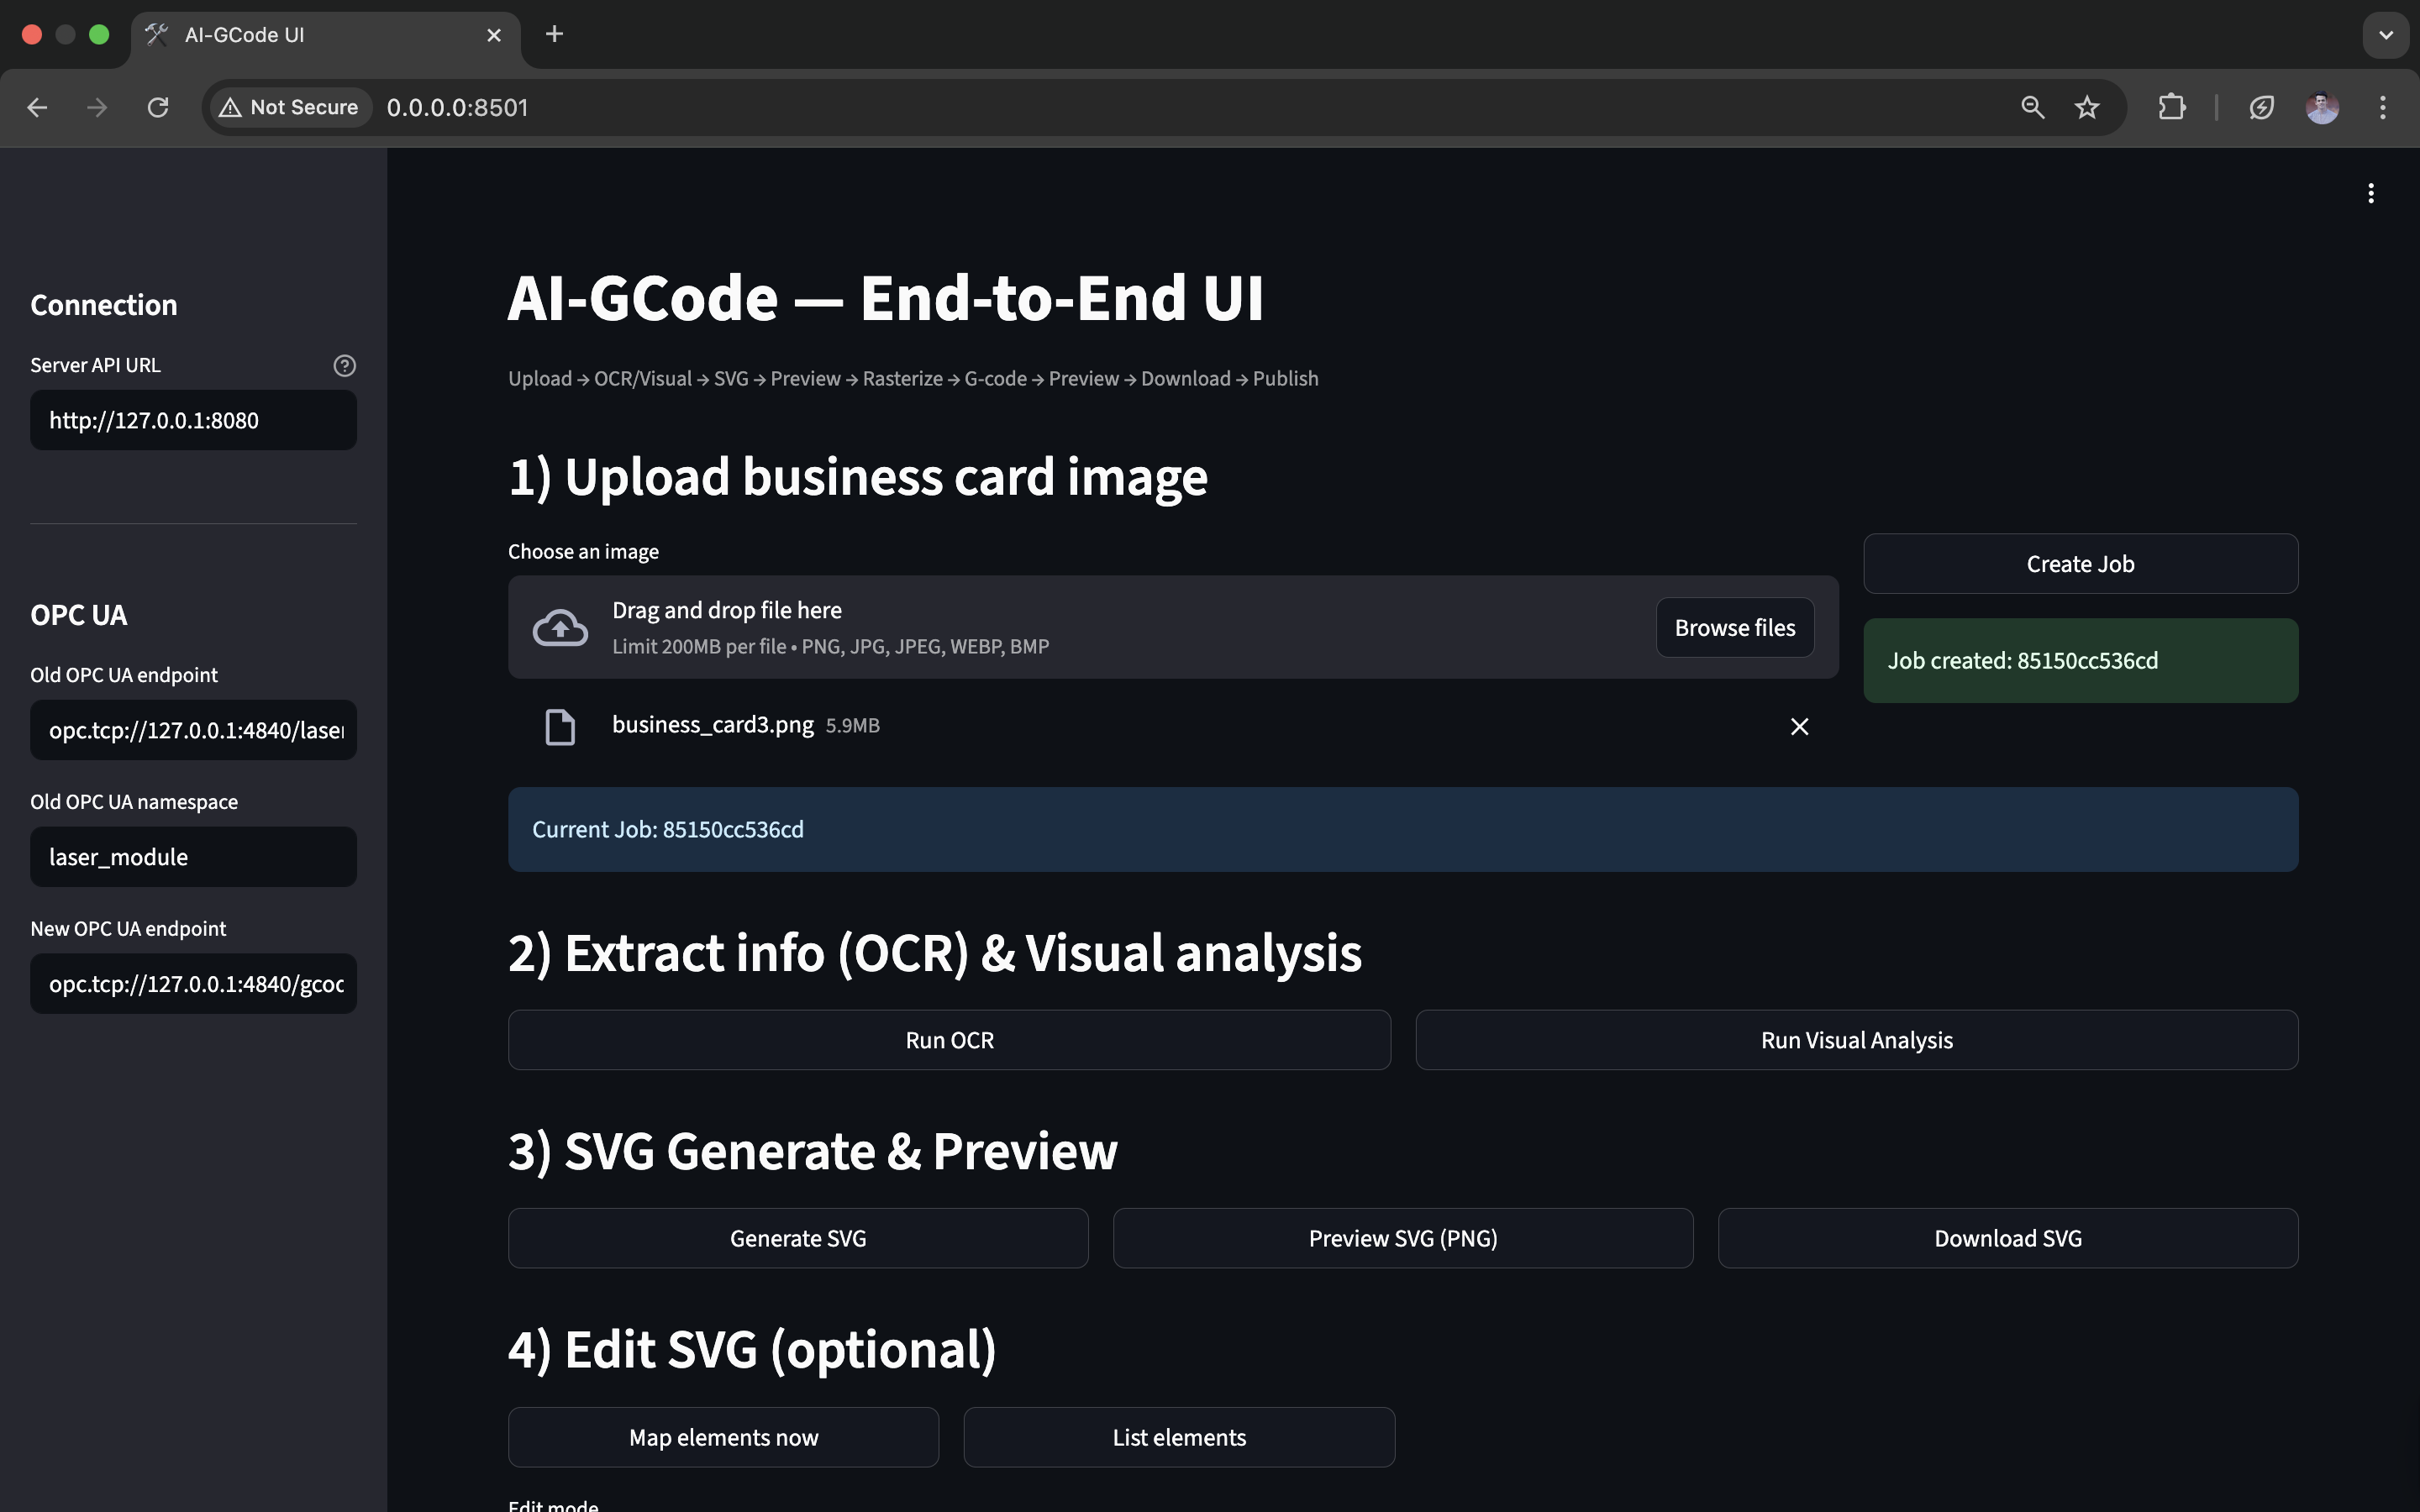
\includegraphics[width=0.9\linewidth]{Images/WebUI.png}
		\caption{Web UI}
		\label{WebUI} 
	\end{center}
\end{figure}

\subsection{API Documentation with FastAPI}
A key feature of the backend \texttt{server\_api.py} is the automatic generation of interactive API documentation as shown in fig.~\ref{API} , provided by the FastAPI framework. Once the server is started with ~\ref{lst:backend}. The documentation can be accessed at:

\begin{lstlisting}[language=bash,caption={API Documentation}, label={lst:APID}]
	http://localhost:8080/docs
\end{lstlisting}

This launches the Swagger UI, an OpenAPI-based interactive interface that lists all available endpoints. Users and developers can:

\begin{itemize}
	\item \textbf{Inspect endpoints:} View the methods implemented in the backend, such as uploading images, generating SVG files, or producing G-code.
	\item \textbf{Test interactively:} Submit requests directly in the browser (e.g., upload a card image and check the JSON output).
	\item \textbf{Validate responses:} Confirm that each endpoint returns the correct output before triggering the full workflow via the Web UI.
\end{itemize}

\begin{figure}
	\begin{center}
		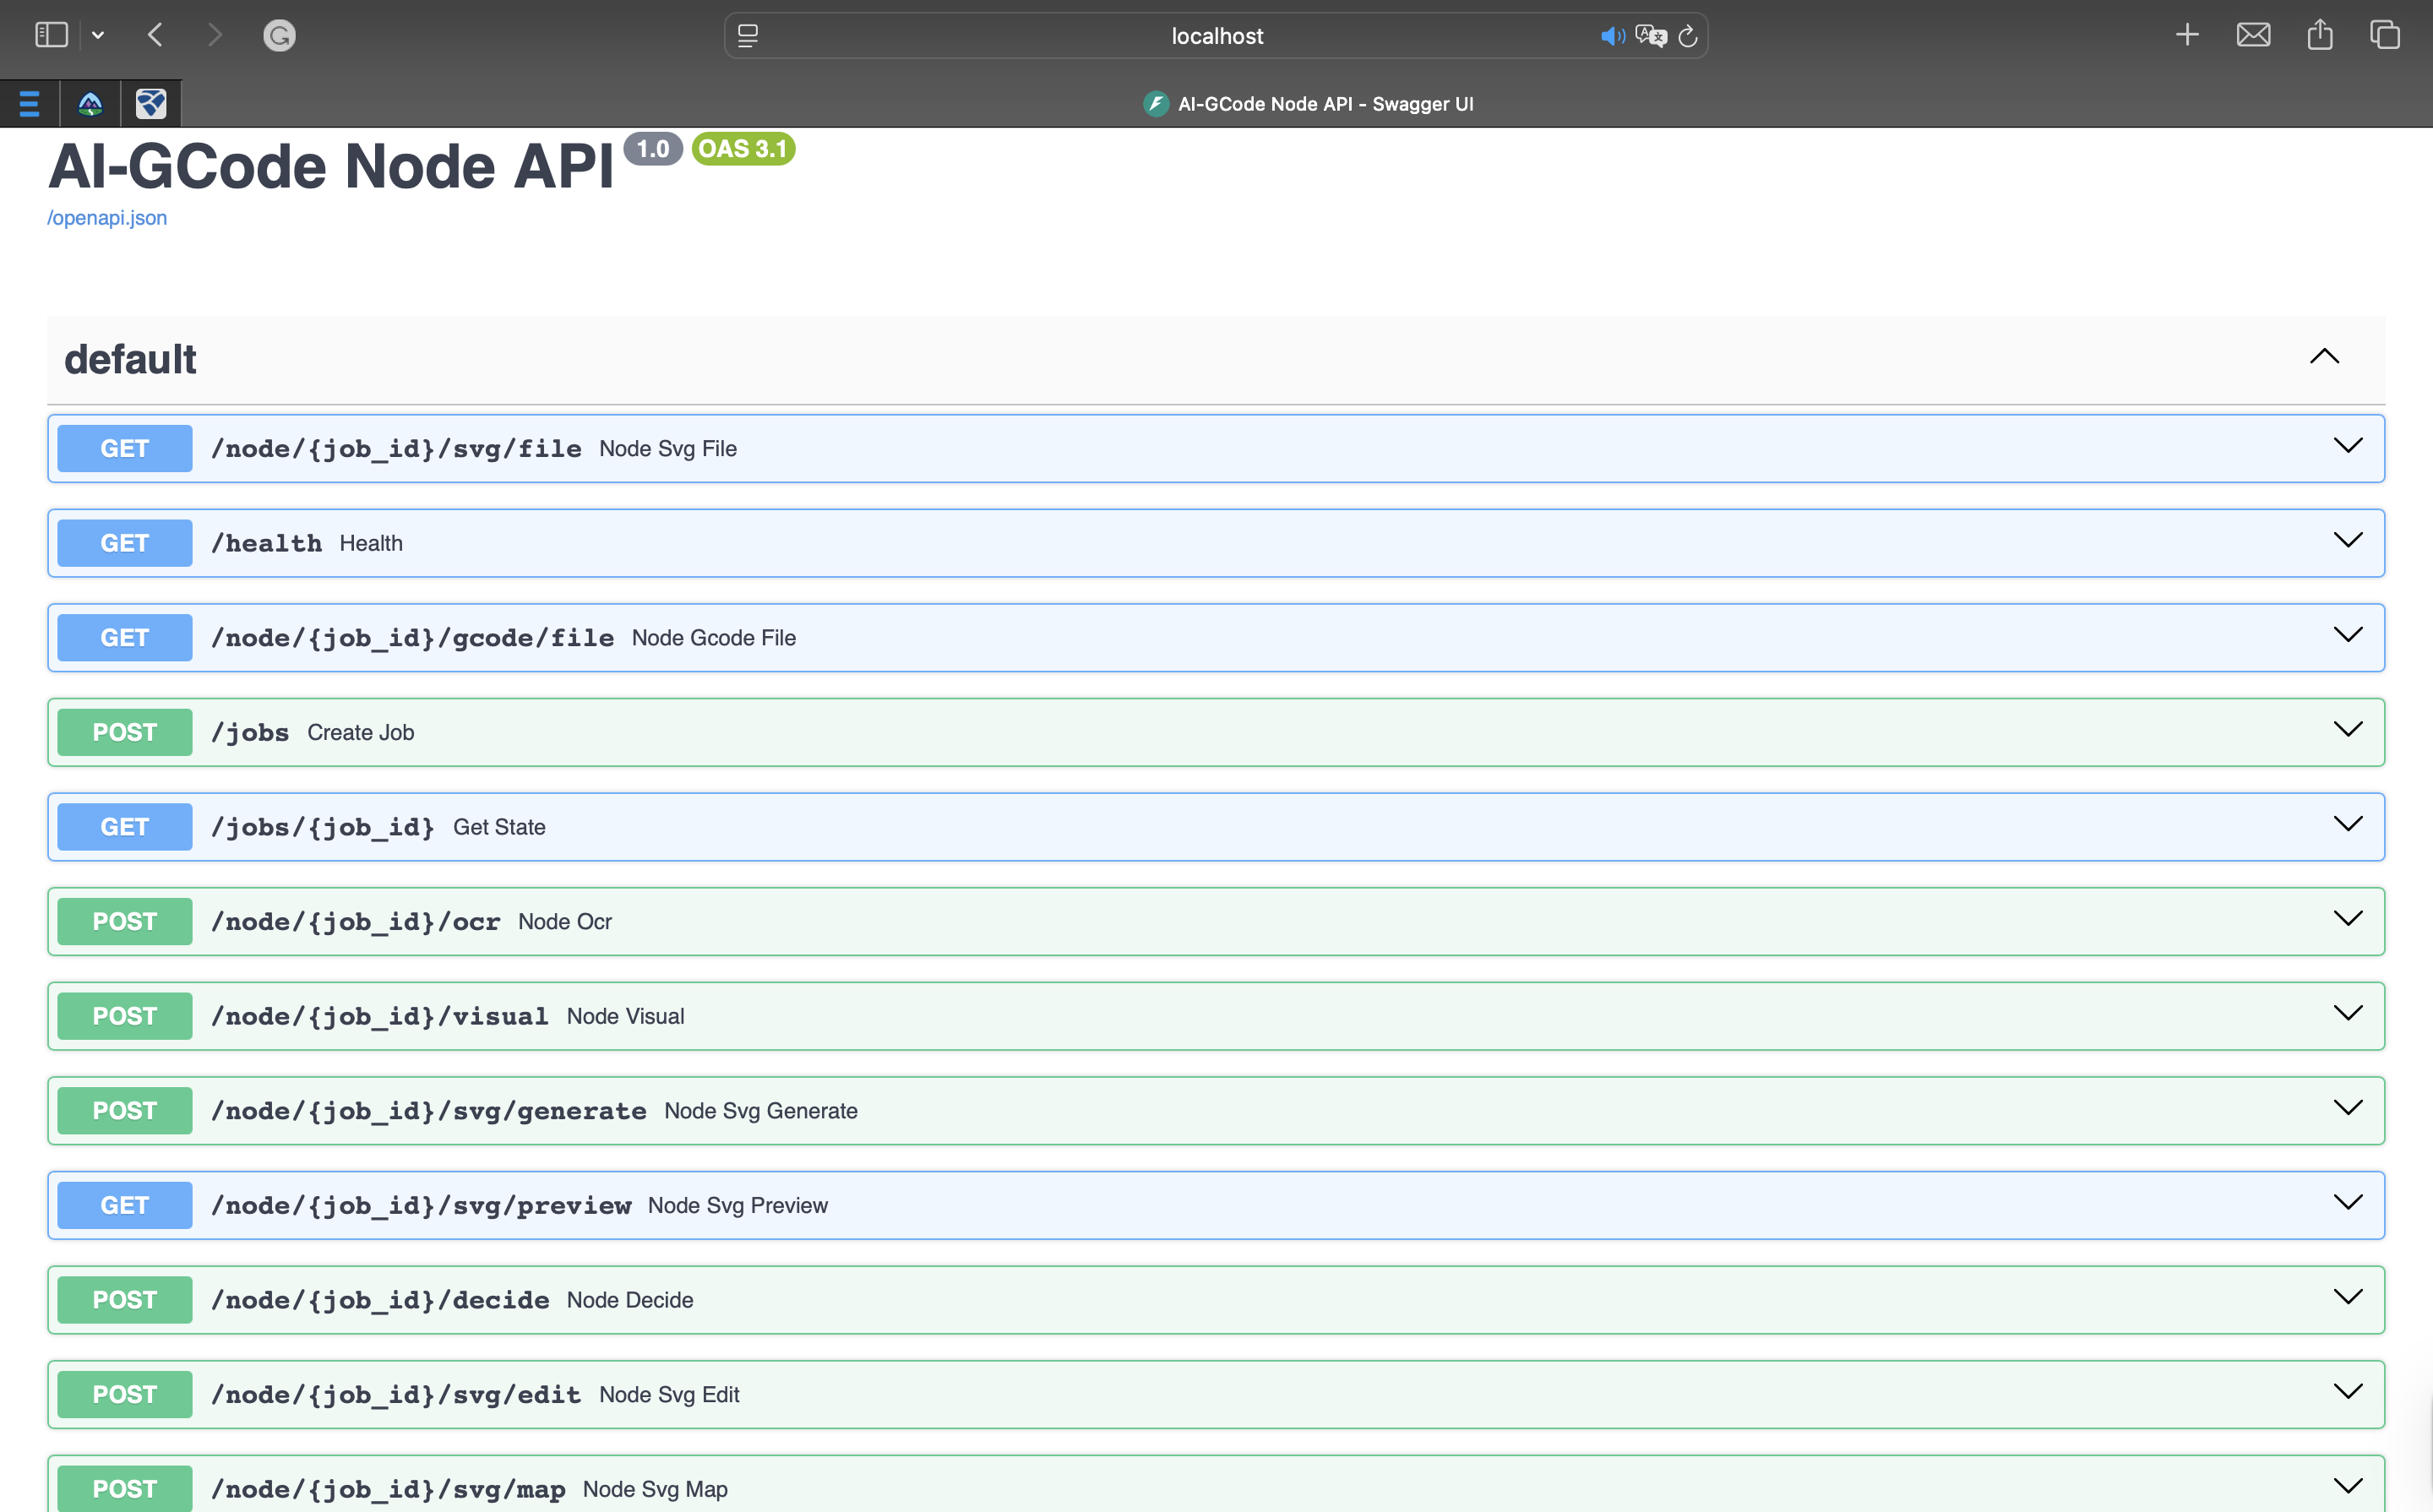
\includegraphics[width=1\linewidth]{Images/API.png}
		\caption{API Documentation}
		\label{API} 
	\end{center}
\end{figure}

This documentation serves both as a developer tool for debugging and as a transparency layer, showing exactly how the Web UI communicates with the backend. Such self-documenting APIs are considered best practice in modern Industry 4.0 software development, as they enhance reproducibility, usability, and integration potential.

\section{OPC UA}
The OPC UA implementation is embedded in the backend files \texttt{server\_api.py, server\_hmi.py, and client\_hmi.py}. The structure follows a typical server–client architecture:
\begin{itemize}
	\item \texttt{server\_api.py:} Hosts variables and methods representing engraving jobs (e.g., job ID, file path, status).
	\item \texttt{server\_hmi.py:} Provides a structured way to interact with OPC UA nodes, enabling monitoring and updating of job status.
	\item \texttt{client\_hmi.py:} Connects to the OPC UA server to retrieve or update information, such as reading the generated G-code file path or confirming job completion.
\end{itemize}


\subsection{Workflow with OPC UA}
\begin{itemize}
	\item After generating the final G-code file, the user specifies the target OPC UA endpoint directly in the Web UI sidebar under the OPC UA Section as shown in the fig ~\ref{WebUI}.
\item In the Digital Factory context, this endpoint corresponds to the HMI server connected to the Laser Engraver Module. The user provides the server’s IP address and the correct namespace URI.
\item Once configured, the backend publishes the file path and relevant job metadata (e.g., job ID, timestamp) to the designated OPC UA server.
\item The OPC UA client then retrieves this information from the server.
\item Finally, the client forwards the engraving job to the Laser Engraver Module in the Digital Factory, where it can be executed as part of the modular production workflow.
\end{itemize}

\section{Docker Integration}
\subsection{Purpose of Dockerisation}
Docker was used to containerise the system in order to simplify deployment, ensure reproducibility, and allow others to run the full AI-GCode-Generation pipeline locally on their own machines without manual setup. By encapsulating all dependencies—such as Python libraries, LangGraph, AI models, and OPC UA modules—within Docker images, the system achieves portability across different operating systems and environments.

\subsection{Implementation}
The project includes a \texttt{Dockerfile} and \texttt{docker-compose.yml} configuration (see repository root). These files define how the environment is built and how different services (backend API, Streamlit UI, and OPC UA integration) are orchestrated together.


\begin{itemize}
	\item \texttt{Dockerfile:} Specifies the base image (Python 3.12), installs required packages from requirements.txt, copies project files, and sets environment variables.
	\item \texttt{docker-compose.yml:} Configures multi-service deployment, including
	\begin{itemize}
		\item \textbf{Backend API container (FastAPI with Uvicorn)}
		\item \textbf{Streamlit UI container}
		\item \textbf{OPC UA service container} (server or client, depending on configuration)
	\end{itemize}
	\item \texttt{.env file:} stores API keys (Fireworks, OpenRouter, LangGraph) and is mounted inside the container for secure configuration. For ensure proper execution:
	\begin{itemize}
		\item The \textbf{.env} file must be in the same directory as  \textbf{docker-compose.yml}.
		\item The \textbf{.env} file should contain all required API keys and must not have any file extensions (e.g., no .txt).
	\end{itemize}
\end{itemize}

\subsection{Workflow with Docker}
\subsubsection{Clone the repository:}

\begin{lstlisting}[language=bash,caption={Clone Repository}, label={lst:text}]
	git clone https://github.com/mahajan-vatsal/AI-GCode-Generation.git
	cd AI-GCode-Generation
\end{lstlisting}
		
\subsubsection{Build the Docker images:}

\begin{lstlisting}[language=bash,caption={Build Image}, label={lst:text}]
		docker-compose build
\end{lstlisting}

\subsubsection{Launch the containers:}

\begin{lstlisting}[language=bash,caption={Launch Container}, label={lst:text}]
		docker-compose up
\end{lstlisting}

\subsubsection{Access the system locally:}

 		\begin{itemize}
 		\item \textbf{Web UI}→ \texttt{http://localhost:8501}
 	\item \textbf{Backend API} → \texttt{http://localhost:8080}
 \end{itemize}
 
This approach enables collaborators to launch the system with a single command, without manually configuring Python environments or dependencies.

\begin{figure}
	\begin{center}
		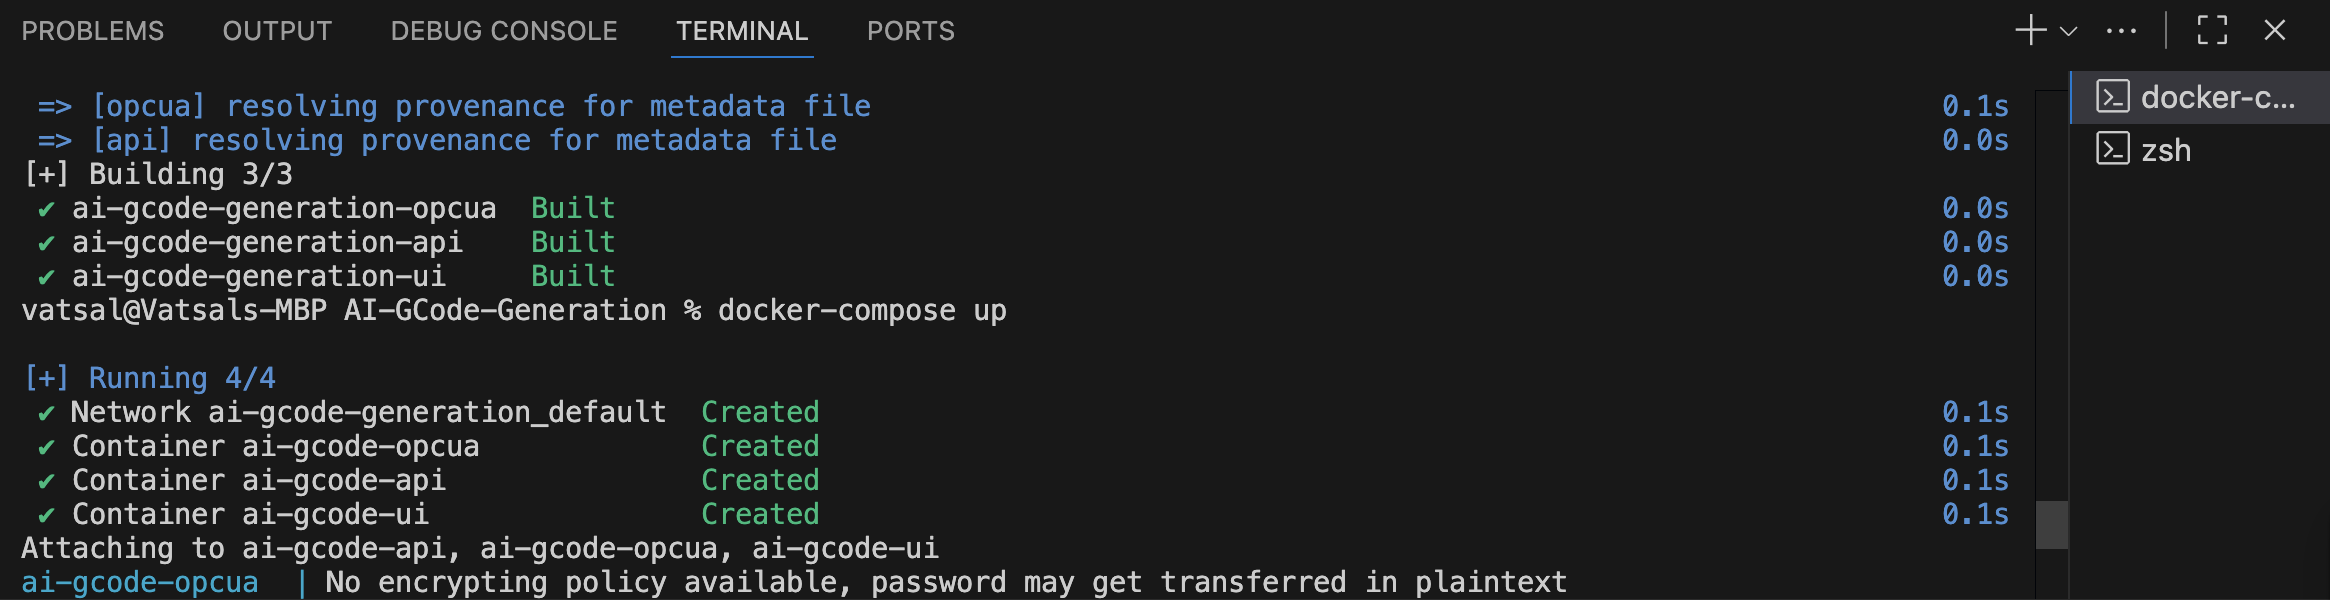
\includegraphics[width=1\linewidth]{Images/dockerT.png}
		\caption{Docker Run}
		\label{DockerT} 
	\end{center}
\end{figure}

\begin{figure}
	\begin{center}
		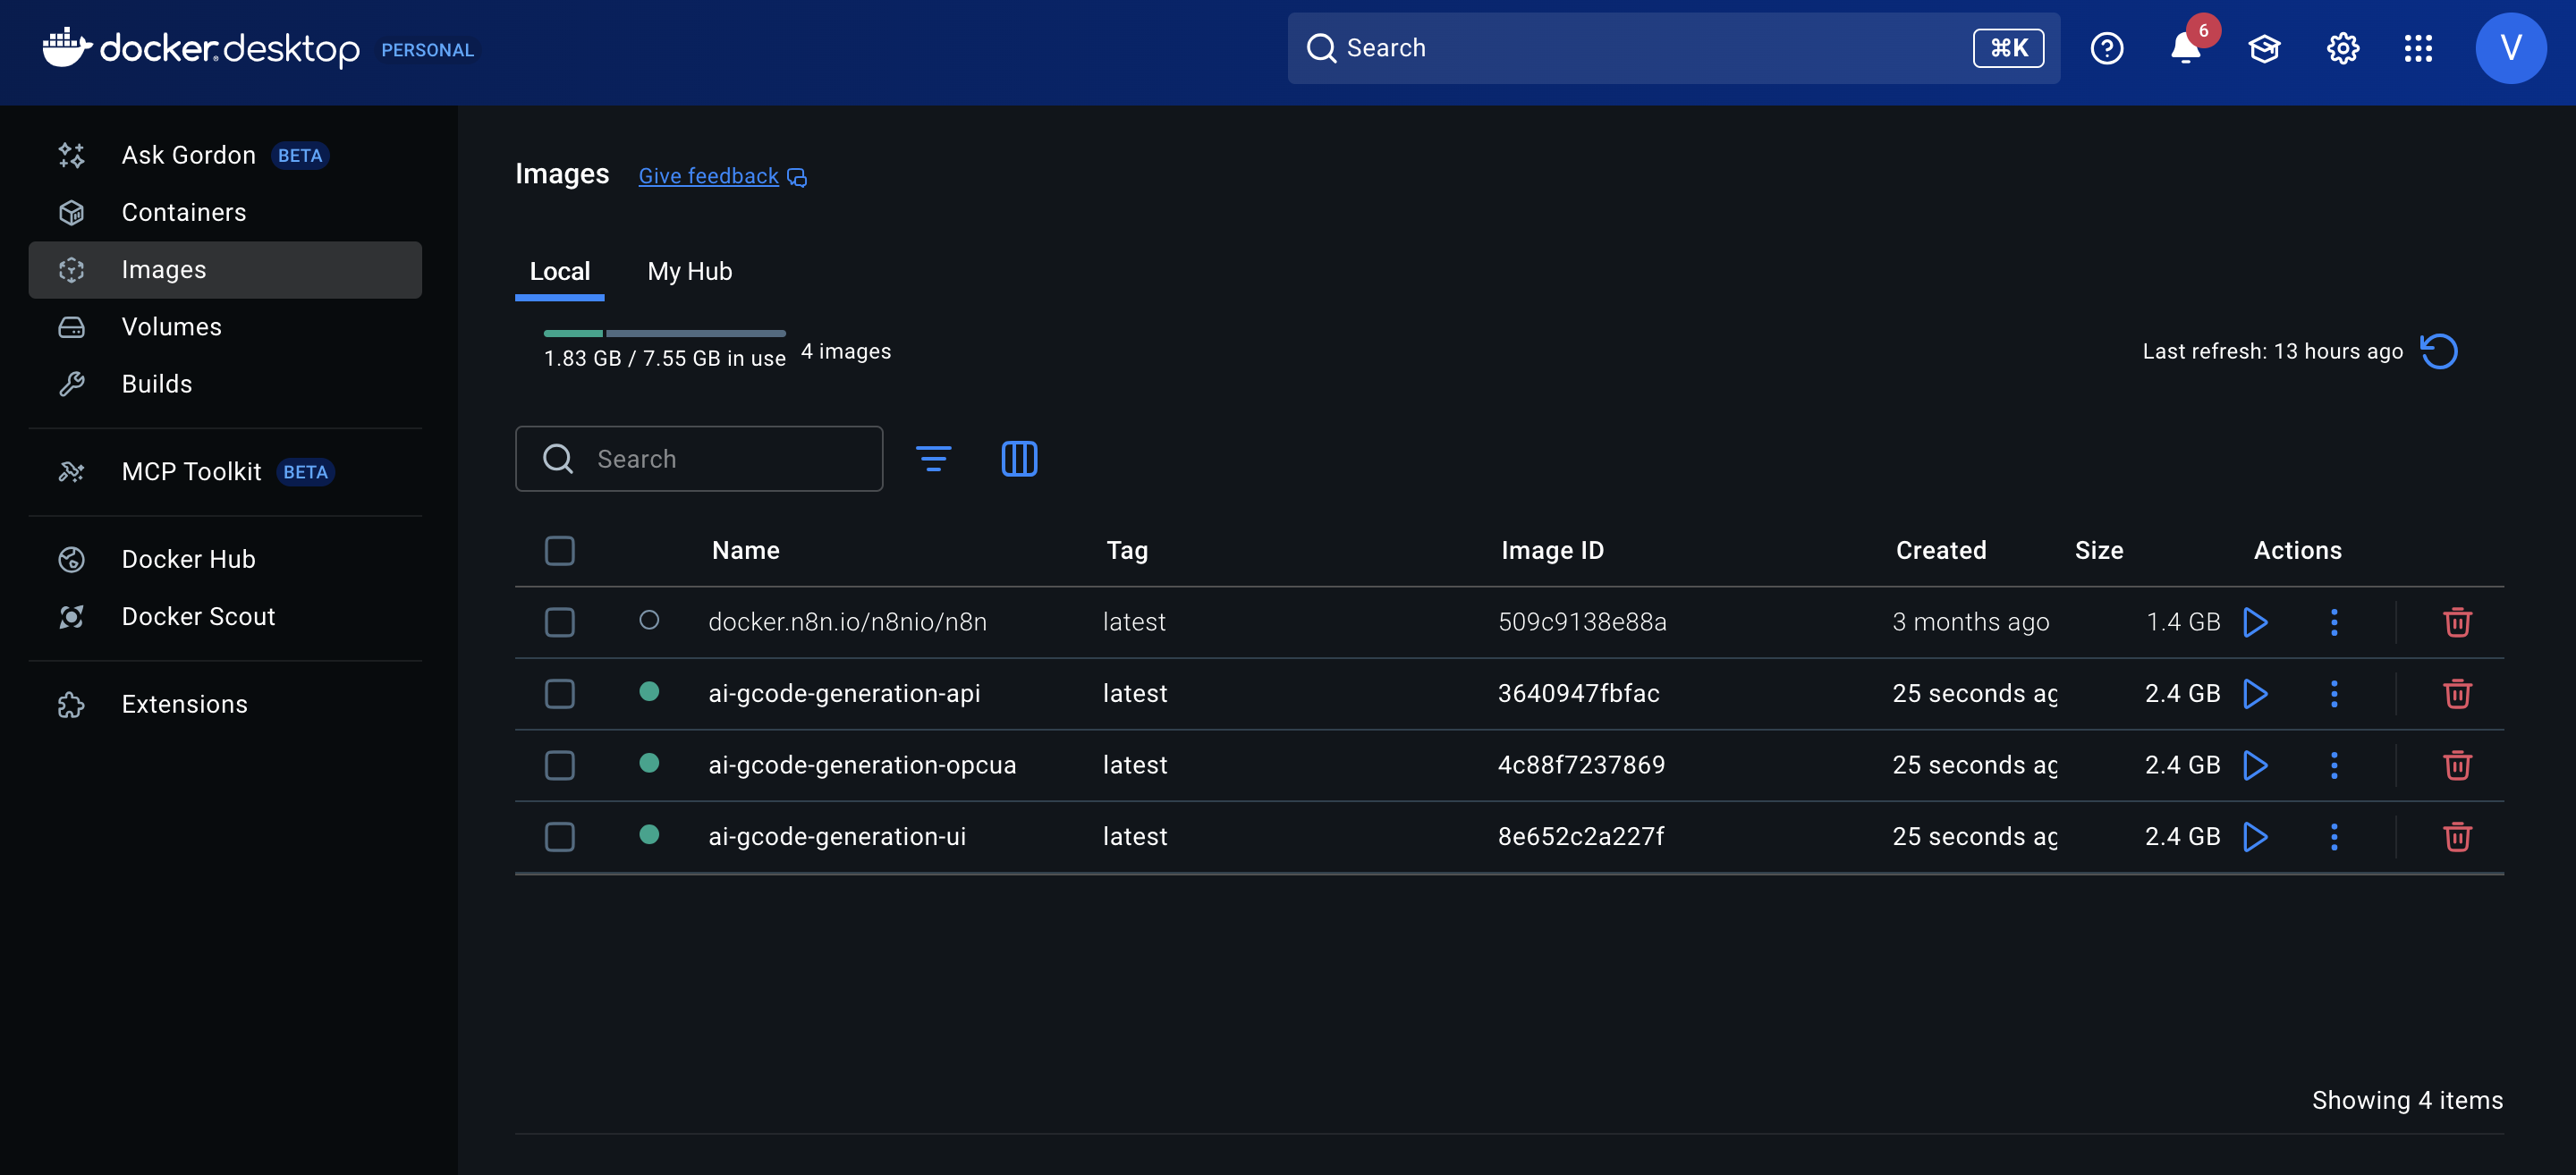
\includegraphics[width=1\linewidth]{Images/docker.png}
		\caption{Docker Desktop}
		\label{Docker} 
	\end{center}
\end{figure}
